\documentclass[11pt]{article}
\usepackage[english]{babel}
\usepackage[utf8]{inputenc}
\usepackage{ifthen}
\selectlanguage{english}
\usepackage[pdftex]{graphicx}
\usepackage{fancyhdr}
\usepackage{subfigure}
\usepackage[hmargin=1in,vmargin=1in]{geometry}
\usepackage{setspace}
\usepackage{url}
%\usepackage{fancyhdr}
%\pagestyle{fancy}
%%% ----------------------------------------------------------------------

%\rfoot{\thepage}
%\cfoot{}
%\lhead{}
\pagestyle{fancy}
\lhead{GSBGEN 390 : Individual Research \\ Sponsoring Professor William Barnett}
\rhead{Pedro Alves Ribeiro Côrte-Real \\ SUID: 005575591}
\lfoot{}
\rfoot{}
\setlength{\headheight}{30pt}

\title{Final Writeup}
\date{June 7, 2011}
\author{Pedro Côrte-Real}

\begin{document}

\thispagestyle{fancy}
\begin{center}
  \textbf{\Large Final Paper}
\end{center}

\section{Introduction}

Open-source development, by its public nature, provides a valuable data source to study how systems are composed and evolve. Previous work on building quantitative measures based on the source are either outdated\cite{sloccount} or target only a specific project\cite{lwnstats,gnomecensus}. The objective of this work was to look at a representative cross-section of open-source software currently being used and extract from it both immediate conclusions and a repeatable method that can be extended for further study. All data and code to produce the analysis and its outputs (including this document) is itself contained within an open-source project\cite{repo}.

\section{Methodology}

The development of open-source software is highly dispersed, so to study a finite set a selection criteria must be established. For the purpose of this study the Ubuntu Linux distribution was used as a reference because it is:
\begin{itemize}
\item Based on and includes the full Debian archive which is the biggest of any Linux distribution
\item Organized as fixed time releases\cite{ubuntureleases} so any given iteration will roughly correspond to a 6 month effort by the whole community\footnote{unless packaging of new versions of released software is lagging behind}
\item Backed by a commercial entity, and so open to the question as to how the small amount of contribution by the parent company can make a difference in the much higher output of the full community
\end{itemize}

Having selected Ubuntu as the basis for comparison the methodology used was to match consecutive versions of the same packages between consecutive iterations of the distribution and calculate relevant metrics:
\begin{itemize}
\item The total lines of code (LOC) in the package, as a proxy for its relative size
\item The total LOC that were actually added and remove to a given package\footnote{altered lines are counted as both an addition and removal, leading to what could be considered a double counting}
\item A measure of churn in the code base defined as the total number of lines changed between the two version divided by the total LOC of the original version as calculated before
\end{itemize}

These two metrics, together with metadata about the packages (e.g., their original source project) forms the basis of the initial results of the research. The results presented were limited to Ubuntu's ``main'' repository, the roughly 3.000 packages that Ubuntu supports directly and are selected from the more than 30.000 that Debian packages. The hope is that by focusing on this selection a representative subset is chosen of what constitutes the most relevant open-source software for at least the desktop and server uses Linux distributions are commonly employed for.

\section{Preliminary Results}

A first analysis\cite{prelimresults} was focused on the relationship between size and churn and how the total amount of mutation in the code base has been evolving over time.

\begin{figure}[htb]
  \begin{center}
    \subfigure[Churn vs Size]{\label{churn:size}\includegraphics[width=80mm]{../generated/sizevschurn/sizevschurn.pdf}}
    \subfigure[Churn per section]{\label{churn:section}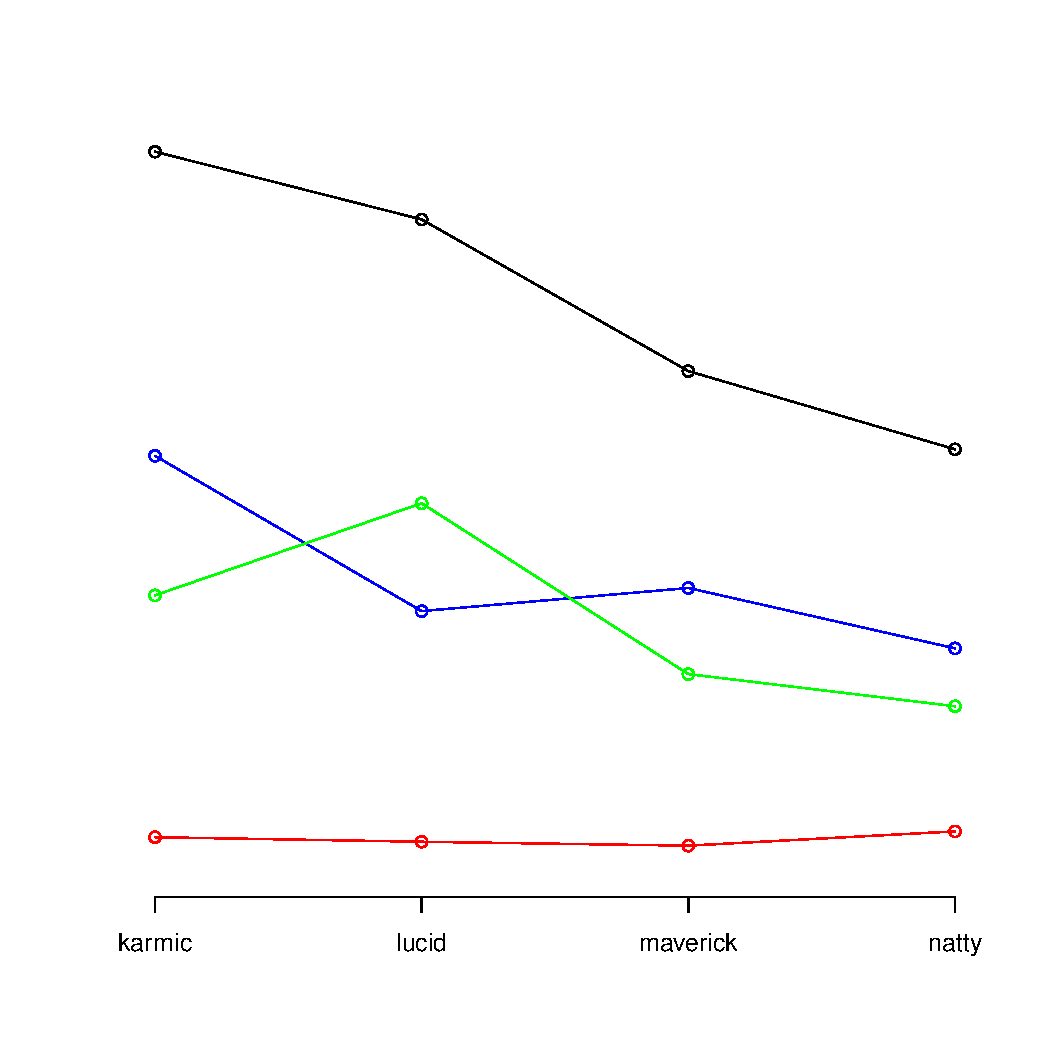
\includegraphics[width=80mm]{../generated/sectionsplit/sectionsplit.pdf}}
  \end{center}
  \caption{Package to package churn in the last four Ubuntu releases}
  \label{fig:churn}
\end{figure}

Figure~\ref{churn:size} shows there is a negative correlation between the size of a given package and the churn it goes through in a given development cycle. The plot is not very convincing but the result is highly statistically significant\footnote{$p < 2 \times 10^{-16}$; Since there are many other factors that explain Churn than total LOC by itself the R-squared is very small at 0.04. This is evident in how the scatter plot does not even hint at what the regression line is}. It is perhaps not particularly surprising that as a package grows bigger more parts of it are mature and the total rate of mutation as a percentage slows. If that explains the full effect then this is not a particularly insightful result. It remains to be checked by future work if controlling for a measure package maturity is enough to eliminate this effect or if there is in fact a negative impact on the rate of mutation from a package growing larger. Software Engineering practice would support this hypothesis, as the complexity of the project makes its evolution harder.

Figure~\ref{churn:section} shows the evolution of the total amount of code changes across the whole distribution. Here the surprising result is that the total amount of mutation of the distribution has been steadily decreasing. On the other hand the absolute numbers are staggering. In just 6 months, just the narrow slice of packages in Ubuntu main has consistently received more than 100M lines of changes. That is 5-10 times the whole Linux kernel, a 20 year old and highly complex piece of software, every 6 months.

The second analysis was focused on the question of how much of the GNU project, started by Richard Stallman, to create a complete Unix replacement, is still present in a modern distribution\cite{gnuinlinux} and how much other projects weigh in on the same metric.

\begin{figure}[htb]
  \begin{center}
    \subfigure[Total]{\label{gnuinlinux:total}\includegraphics[height=60mm]{../generated/gnuinlinux/totalsplit.pdf}}
    \subfigure[GNU software]{\label{gnuinlinux:gnu}\includegraphics[height=60mm]{../generated/gnuinlinux/gnusplit.pdf}}
  \end{center}
  \caption{LOC split of projects in Ubuntu natty's main repository}
  \label{fig:gnuinlinux}
\end{figure}

Figure~\ref{gnuinlinux:total} shows the split in total size of Ubuntu packages divided by their originating projects. It is interesting to discover that the kernel and its accompanying utilities amounts to a fraction very similar to GNU's. Perhaps more surprising is that almost 60\% of the distribution is sourced from very small projects, each often producing a single application.

Figure~\ref{gnuinlinux:gnu} shows the projects that compose the GNU slice. With the notable exception of \texttt{gdb} all the large GNU projects have viable and popular alternatives in active use. This together with the high percentage of packages sourced from small projects argues for the decreasing importance of large umbrella projects, instead replaced by distributions as the most relevant aggregator in the supply chain between original developers and end-users.

\section{Future Work}

The work presented is but a proof of concept of what can be done with the source code as a data source. Potential avenues of further refinement and extension of the work are (from small to large):
\begin{itemize}
\item Improve the methodology of how churn and LOC are calculated to better account for the differing types of programming languages
\item Explore using a weighted sum of LOC as a better size metric, correcting for the relative verbosity of programming languages
\item Creating a maturity variable based on the openly accessible bug database for the same packages
\item Use the Ubuntu/Debian package popularity results to relate the effort put into packages and their changes in popularity with end-users
\item Do comparisons based on other unrelated Linux distributions such as Fedora and RedHat
\item Re-purpose the same types of analysis for the Debian archive and see if Ubuntu's corporate sponsor (Canonical) can be observed to have a significant effect
\item Look at finer grained data from the version control systems that are used to store the code for the project, allowing analysis of the micro-aspects of the evolution, instead of the relatively large 6 month steps studied here
\item Explore code repository communities such as GitHub and its dynamics as a social graph on top of code repositories
\item Obtain access to and perform similar analysis on large close-sourced code bases as the Windows or OS X sources
\end{itemize}

\section{Conclusion}

Source code is itself good quality data; programmers produce it in its original form so it is directly a human output; it is unambiguously and mechanically translated into final usable software so it is a complete definition; it is usually stored in systems that record not only its most recent version but also a full record of its evolution so it includes an inherent time series of mutation. 

The conclusions extracted so far are still tentative and incomplete. The most interesting achievement of this work has been the production of a first base of repeatable and fully automated analysis that can be used to target existing code bases and extract from them meaningful metrics. 

The analysis made are fully defined in source code, with no manual steps. This allows for the same kind of incremental approach that is used to build complex systems to be used to further the study in this area, while at the same time retaining a complete record of all the steps taken. It has been invaluable throughout the project to be able to go back to previous versions of the work and understand why modifications were having unexpected results. In a lot of ways the codification of the complete method of analysis replaces the lab notebook and makes repetition of previous experiments trivial.

\newpage
\begin{thebibliography}{9}

\bibitem{sloccount}
David A. Wheeler,
\emph{More Than a Gigabuck: Estimating GNU/Linux's Size}\\
\url{http://www.dwheeler.com/sloc/redhat71-v1/redhat71sloc.html}\\
June 30, 2001 (updated July 29, 2002)

\bibitem{lwnstats}
Jonathan Corbet,
\emph{2.6.39 development statistics}\\
\url{https://lwn.net/Articles/442229/}\\
May 10, 2011

\bibitem{gnomecensus}
Neary Consulting,
\emph{The GNOME Census: Who writes GNOME?}\\
\url{http://www.neary-consulting.com/docs/GNOME_Census.pdf}\\
July 28, 2010

\bibitem{repo}
\emph{Source repository}\\
\url{https://github.com/pedrocr/codecomp}

\bibitem{ubuntureleases}
\emph{List of Ubuntu releases}\\
\url{https://wiki.ubuntu.com/Releases}

\bibitem{prelimresults}
Pedro Côrte-Real,
\emph{Preliminary Results from Open Source Evolution Analysis}\\
\url{http://pedrocr.net/text/preliminary-results-open-source-evolution}\\
May 12 2011

\bibitem{gnuinlinux}
Pedro Côrte-Real,
\emph{How much GNU is there in GNU/Linux?}\\
\url{http://pedrocr.net/text/how-much-gnu-in-gnu-linux}\\
May 31 2011

\end{thebibliography}

\end{document}
